\documentclass[11pt]{standalone}
\usepackage{amssymb}
\usepackage{amsmath}
\usepackage[no-math]{fontspec}
\usepackage{unicode-math}
\usepackage{libertinus}
\usepackage{pgf,xcolor}
\usepackage{tikz}
\usetikzlibrary{arrows.meta, backgrounds}
\usepackage{pgfplots}
\pgfplotsset{compat=newest}
\usepgfplotslibrary{groupplots}

\definecolor{my_darkgray}{HTML}{484949}
\definecolor{my_lightgray}{HTML}{F3F4F4}
\definecolor{my_darkblue}{HTML}{005A94}
\definecolor{my_lightblue}{HTML}{CCDEE9}
\definecolor{my_yellow}{HTML}{FFEC7F}
\definecolor{my_red}{HTML}{E60000}
\definecolor{my_orange}{HTML}{E87846}

\begin{document}
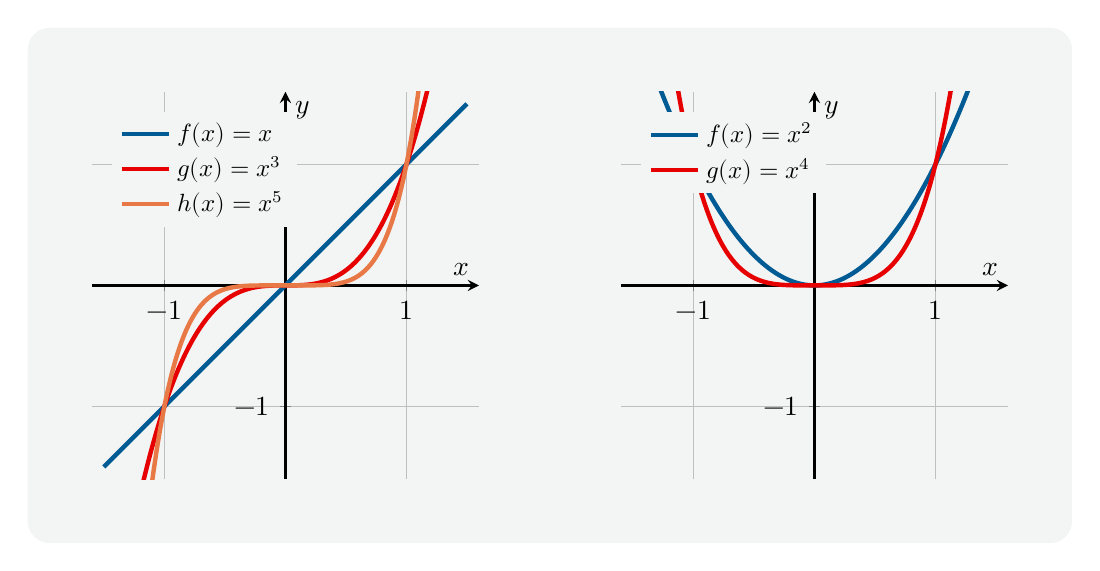
\begin{tikzpicture}[
    show background rectangle,
    background rectangle/.style={fill=my_lightgray, rounded corners=8pt},
    inner frame sep=0.8cm
]
\begin{groupplot}[
    group style={
        group size=2 by 1,
        horizontal sep=1.8cm,
    },
    % Shared axis style
    axis lines=center,
    xlabel={$x$},
    ylabel={$y$},
    height=6.5cm, width=6.5cm,
    xmin=-1.6, xmax=1.6,
    ymin=-1.6, ymax=1.6,
    xtick={-1, 0, 1},
    ytick={-1, 0, 1},
    grid=both,
    axis line style={thick},
    legend style={
        font=\small,
        at={(0.05, 0.95)},
        anchor=north west,
        draw=none,
        fill=my_lightgray,
    },
    legend cell align=left,
]

% Left panel: odd exponents — point-symmetric about the origin
\nextgroupplot
\addplot[draw=my_darkblue, samples=300, ultra thick, domain=-1.5:1.5]{x};
\addlegendentry{$f(x)=x$}
\addplot[draw=my_red, samples=300, ultra thick, domain=-1.5:1.5]{x^3};
\addlegendentry{$g(x)=x^3$}
\addplot[draw=my_orange, samples=300, ultra thick, domain=-1.5:1.5]{x^5};
\addlegendentry{$h(x)=x^5$}

% Right panel: even exponents — symmetric about the y-axis
\nextgroupplot
\addplot[draw=my_darkblue, samples=300, ultra thick, domain=-1.5:1.5]{x^2};
\addlegendentry{$f(x)=x^2$}
\addplot[draw=my_red, samples=300, ultra thick, domain=-1.5:1.5]{x^4};
\addlegendentry{$g(x)=x^4$}

\end{groupplot}
\end{tikzpicture}
\end{document}
